% Options for packages loaded elsewhere
\PassOptionsToPackage{unicode}{hyperref}
\PassOptionsToPackage{hyphens}{url}
\PassOptionsToPackage{dvipsnames,svgnames,x11names}{xcolor}
%
\documentclass[
  12pt,
  letterpaper,
  DIV=11,
  numbers=noendperiod]{scrartcl}

\usepackage{amsmath,amssymb}
\usepackage{setspace}
\usepackage{iftex}
\ifPDFTeX
  \usepackage[T1]{fontenc}
  \usepackage[utf8]{inputenc}
  \usepackage{textcomp} % provide euro and other symbols
\else % if luatex or xetex
  \usepackage{unicode-math}
  \defaultfontfeatures{Scale=MatchLowercase}
  \defaultfontfeatures[\rmfamily]{Ligatures=TeX,Scale=1}
\fi
\usepackage{lmodern}
\ifPDFTeX\else  
    % xetex/luatex font selection
  \setmainfont[Scale = MatchLowercase]{Scala Pro}
  \setsansfont[]{Scala Sans Pro}
\fi
% Use upquote if available, for straight quotes in verbatim environments
\IfFileExists{upquote.sty}{\usepackage{upquote}}{}
\IfFileExists{microtype.sty}{% use microtype if available
  \usepackage[]{microtype}
  \UseMicrotypeSet[protrusion]{basicmath} % disable protrusion for tt fonts
}{}
\makeatletter
\@ifundefined{KOMAClassName}{% if non-KOMA class
  \IfFileExists{parskip.sty}{%
    \usepackage{parskip}
  }{% else
    \setlength{\parindent}{0pt}
    \setlength{\parskip}{6pt plus 2pt minus 1pt}}
}{% if KOMA class
  \KOMAoptions{parskip=half}}
\makeatother
\usepackage{xcolor}
\usepackage[margin=25mm]{geometry}
\setlength{\emergencystretch}{3em} % prevent overfull lines
\setcounter{secnumdepth}{-\maxdimen} % remove section numbering
% Make \paragraph and \subparagraph free-standing
\ifx\paragraph\undefined\else
  \let\oldparagraph\paragraph
  \renewcommand{\paragraph}[1]{\oldparagraph{#1}\mbox{}}
\fi
\ifx\subparagraph\undefined\else
  \let\oldsubparagraph\subparagraph
  \renewcommand{\subparagraph}[1]{\oldsubparagraph{#1}\mbox{}}
\fi


\providecommand{\tightlist}{%
  \setlength{\itemsep}{0pt}\setlength{\parskip}{0pt}}\usepackage{longtable,booktabs,array}
\usepackage{calc} % for calculating minipage widths
% Correct order of tables after \paragraph or \subparagraph
\usepackage{etoolbox}
\makeatletter
\patchcmd\longtable{\par}{\if@noskipsec\mbox{}\fi\par}{}{}
\makeatother
% Allow footnotes in longtable head/foot
\IfFileExists{footnotehyper.sty}{\usepackage{footnotehyper}}{\usepackage{footnote}}
\makesavenoteenv{longtable}
\usepackage{graphicx}
\makeatletter
\def\maxwidth{\ifdim\Gin@nat@width>\linewidth\linewidth\else\Gin@nat@width\fi}
\def\maxheight{\ifdim\Gin@nat@height>\textheight\textheight\else\Gin@nat@height\fi}
\makeatother
% Scale images if necessary, so that they will not overflow the page
% margins by default, and it is still possible to overwrite the defaults
% using explicit options in \includegraphics[width, height, ...]{}
\setkeys{Gin}{width=\maxwidth,height=\maxheight,keepaspectratio}
% Set default figure placement to htbp
\makeatletter
\def\fps@figure{htbp}
\makeatother

\usepackage{fancyhdr}
\usepackage{titling}
\pagestyle{fancy}
\pagenumbering{gobble}
\fancyhf{}
\renewcommand\maketitle{
  \fancyhead[C]{
    \thetitle
    \ifx \theauthor\empty  \else \ – \theauthor \fi
    \ifx \thedate\empty  \else \ – \thedate \ \fi
  }
}
\fancyfoot[C]{\thepage}
\KOMAoption{captions}{tableheading}
\makeatletter
\@ifpackageloaded{caption}{}{\usepackage{caption}}
\AtBeginDocument{%
\ifdefined\contentsname
  \renewcommand*\contentsname{Table of contents}
\else
  \newcommand\contentsname{Table of contents}
\fi
\ifdefined\listfigurename
  \renewcommand*\listfigurename{List of Figures}
\else
  \newcommand\listfigurename{List of Figures}
\fi
\ifdefined\listtablename
  \renewcommand*\listtablename{List of Tables}
\else
  \newcommand\listtablename{List of Tables}
\fi
\ifdefined\figurename
  \renewcommand*\figurename{Figure}
\else
  \newcommand\figurename{Figure}
\fi
\ifdefined\tablename
  \renewcommand*\tablename{Table}
\else
  \newcommand\tablename{Table}
\fi
}
\@ifpackageloaded{float}{}{\usepackage{float}}
\floatstyle{ruled}
\@ifundefined{c@chapter}{\newfloat{codelisting}{h}{lop}}{\newfloat{codelisting}{h}{lop}[chapter]}
\floatname{codelisting}{Listing}
\newcommand*\listoflistings{\listof{codelisting}{List of Listings}}
\makeatother
\makeatletter
\makeatother
\makeatletter
\@ifpackageloaded{caption}{}{\usepackage{caption}}
\@ifpackageloaded{subcaption}{}{\usepackage{subcaption}}
\makeatother
\ifLuaTeX
  \usepackage{selnolig}  % disable illegal ligatures
\fi
\IfFileExists{bookmark.sty}{\usepackage{bookmark}}{\usepackage{hyperref}}
\IfFileExists{xurl.sty}{\usepackage{xurl}}{} % add URL line breaks if available
\urlstyle{same} % disable monospaced font for URLs
\hypersetup{
  pdftitle={Final Exam},
  pdfauthor={Phil 444},
  colorlinks=true,
  linkcolor={black},
  filecolor={Maroon},
  citecolor={Blue},
  urlcolor={Blue},
  pdfcreator={LaTeX via pandoc}}

\title{Final Exam}
\author{Phil 444}
\date{2024-04-26}

\begin{document}
\maketitle

\setstretch{1.2}
Name: \dotfill

Q1 - Describe an example where Sen's Condition L (Liberalism) and
Condition P (Pareto) conflict.

\vspace{0.3cm} \dotfill

\vspace{0.3cm} \dotfill

\vspace{0.3cm} \dotfill

\vspace{0.3cm} \dotfill

\vspace{0.3cm} \dotfill

\vspace{0.3cm} \dotfill

\vspace{0.3cm} \dotfill

\vspace{0.3cm} \dotfill

\vspace{0.3cm} \dotfill

\vspace{0.3cm} \dotfill

\vspace{0.3cm} \dotfill

\vspace{0.3cm} \dotfill

\vspace{0.3cm} \dotfill

\vspace{0.3cm} \dotfill

\vspace{0.3cm} \dotfill

\vspace{0.3cm} \dotfill

\vspace{0.3cm} \dotfill

\vspace{0.3cm} \dotfill

\newpage

Q2 - Describe an example of a \textbf{focal point} in Schelling's sense.

\vspace{0.3cm} \dotfill

\vspace{0.3cm} \dotfill

\vspace{0.3cm} \dotfill

\vspace{0.3cm} \dotfill

\vspace{0.3cm} \dotfill

\vspace{0.3cm} \dotfill

\vspace{0.3cm} \dotfill

\vspace{0.3cm} \dotfill

\vspace{0.3cm} \dotfill

\vspace{0.3cm} \dotfill

\vspace{0.3cm} \dotfill

\vspace{0.3cm} \dotfill

\vspace{0.3cm} \dotfill

\vspace{0.3cm} \dotfill

\vspace{0.3cm} \dotfill

\vspace{0.3cm} \dotfill

\vspace{0.3cm} \dotfill

\vspace{0.3cm} \dotfill

\vspace{0.3cm} \dotfill

\newpage

Q3 - What is the difference between weak dominance and strict dominance?
Describe an example where the two notions come apart.

\vspace{0.3cm} \dotfill

\vspace{0.3cm} \dotfill

\vspace{0.3cm} \dotfill

\vspace{0.3cm} \dotfill

\vspace{0.3cm} \dotfill

\vspace{0.3cm} \dotfill

\vspace{0.3cm} \dotfill

\vspace{0.3cm} \dotfill

\vspace{0.3cm} \dotfill

\vspace{0.3cm} \dotfill

\vspace{0.3cm} \dotfill

\vspace{0.3cm} \dotfill

\vspace{1cm}

\begin{longtable}[]{@{}ccc@{}}
\toprule\noalign{}
& ~~~~~~~~~\textbf{Left}~~~~~~~~~ & ~~~~~~~~~\textbf{Right}~~~~~~~~~ \\
\midrule\noalign{}
\endhead
\bottomrule\noalign{}
\endlastfoot
& & \\
\textbf{Up} & & \\
& & \\
\textbf{Down} & & \\
& & \\
\end{longtable}

\newpage

Q4 - In this table, what will be the result if both players use iterated
deletion of strictly dominated strategies to decide what to do? (In each
cell, Row's payouts are first, and Column's are second.)

\begin{longtable}[]{@{}ccccc@{}}
\toprule\noalign{}
& \textbf{W} & \textbf{X} & \textbf{Y} & \textbf{Z} \\
\midrule\noalign{}
\endhead
\bottomrule\noalign{}
\endlastfoot
\textbf{A} & 6,3 & 0,4 & 2,7 & 1,3 \\
\textbf{B} & 5,5 & 5,6 & 2,3 & 5,8 \\
\textbf{C} & 2,2 & 3,7 & 7,2 & 3,5 \\
\textbf{D} & 4,7 & 0,4 & 1,6 & 2,2 \\
\end{longtable}

Row's move: \dotfill

Column's move: \dotfill

Use the space below for workings

\newpage

Q5 - In this tree, what will be the result if all players uses backward
induction to solve the problem? (At each terminal node, the payouts are
player 1's, then player 2's, then player 3's. Each player moves once;
first player 1, then player 2, then player 3.)

\vspace{1cm}

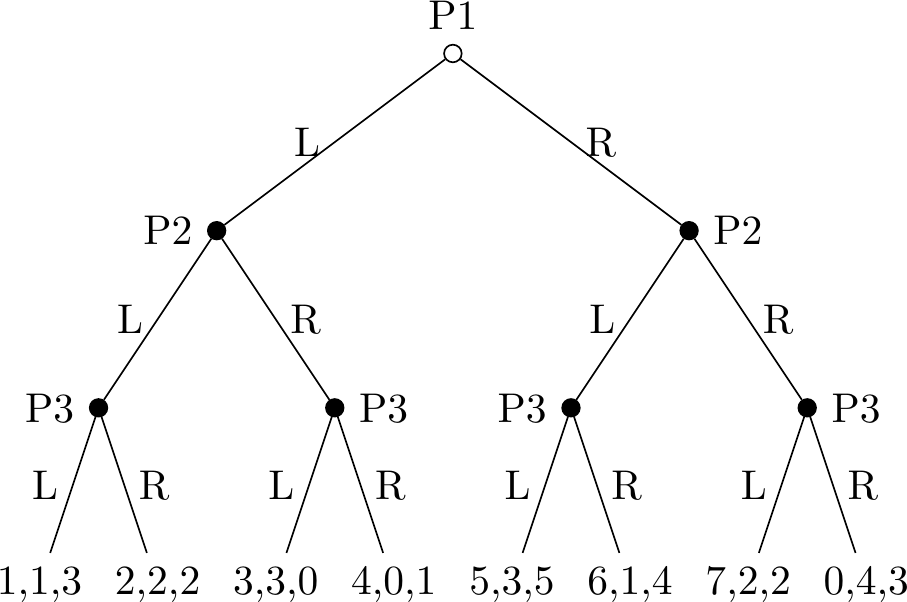
\includegraphics[width=1\textwidth,height=\textheight]{fig-back-1.png}

\vspace{1cm}

P1's move: \dotfill

P2's move: \dotfill

P3's move: \dotfill

P1's payout: \dotfill

P2's payout: \dotfill

P3's payout: \dotfill

\newpage

Q6 - What is the human capital theory of the explanation of the college
wage premium? Describe one objection to it. (You do not have to answer
the objection.)

\vspace{0.3cm} \dotfill

\vspace{0.3cm} \dotfill

\vspace{0.3cm} \dotfill

\vspace{0.3cm} \dotfill

\vspace{0.3cm} \dotfill

\vspace{0.3cm} \dotfill

\vspace{0.3cm} \dotfill

\vspace{0.3cm} \dotfill

\vspace{0.3cm} \dotfill

\vspace{0.3cm} \dotfill

\vspace{0.3cm} \dotfill

\vspace{0.3cm} \dotfill

\vspace{0.3cm} \dotfill

\vspace{0.3cm} \dotfill

\vspace{0.3cm} \dotfill

\vspace{0.3cm} \dotfill

\vspace{0.3cm} \dotfill

\vspace{0.3cm} \dotfill

\newpage

Blank page for extra writing, working out. Please be clear on earlier
pages if part of your answer runs onto these pages.



\end{document}
